\chapter{Arhitektura i dizajn sustava}
		
		Oblikovanje arhitekture i dizajna sustava jedno je od temeljnih i najvažnijih faza razvoja programske potpore. Uključuje glavna pravila i strukture sustava te se sve dalje izgrađuje na osnovi te arhitekture. Upravo zbog toga je ključan faktor u uspješnosti projekta, cijeni i težini izrade te održavanja. 
		
		Za našu aplikaciju odabrali smo objektno orijentiranu arhitekturu jer se pokazala kao najprikladnija za kompleksnu više-korisničku aplikaciju. Kako bi cilj omogućavanja što lakšeg i šireg korištenja naše aplikacije bio ispunjen, odabrali smo izradu web aplikacije kojoj će korisnici moći pristupiti s bilo kojeg uređaja s web preglednikom i  spojenim na mrežu.
		
		Na slici su vidljivi podsustavi klijent-poslužitelj arhitekture sustava. Komunikacija između web preglednika i web poslužitelja odvija se putem HTTP protokola.
	
		\begin{figure}[H]
			\centering
			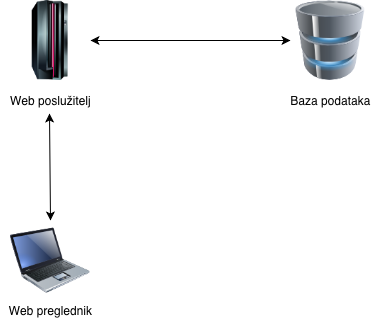
\includegraphics[scale=0.4]{slike/ArhSustav.png}
			\caption{Arhitektura sustava}
		\end{figure}

		\underline{Web preglednik} je program putem kojega korisnik pristupa web-aplikaciji, šalje zahtjeve web poslužitelju i prikazuje vizualnu interpretaciju odgovora.
		
		\underline{Web poslužitelj} prima zahtjeve od korisnika i prosljeđuje ih web aplikaciji koja je pokrenuta na njemu, a odgovore na taj zahtjev, koje dobije od web aplikacije, prosljeđuje natrag web pregledniku korisnika.
		
		\underline{Web aplikacija} na osnovu logike sustava, zahtjeva korisnika i podataka iz baze podataka generira odgovor na zahtjev korisnika.
		
		Objektno orijentirana paradigma je način modeliranja sustava u kojem su osnova izgradnje objekti i modularnost, a osnovni elementi su:
		
			\begin{packed_item}
			
			\item \textbf{Objekt }- primjerak razreda, odnosno smislene cjeline, sadrži vlastite atribute i metode
			\item \textbf {Nasljeđivanje }- mogućnost preuzimanja metoda od razreda-roditelja ili nadjačavanje istih vlastitim proširenjima
			\item \textbf{Polimorfizam }- moguće je postojanje metoda istog imena, a različitih atributa i funkcionalnosti 
			\end{packed_item}
		
		Oblikovanje navedene arhitekture pratit će MVC(Model-View-Controller) obrazac koji se sastoji od:
		
			\begin{packed_item}
				\item \textbf{Model }- struktura za spremanje i upravljanje objektima i podacima
				\item \textbf{View }- komponenta za vizualni prikaz podataka korisniku
				\item \textbf{Controller }- sadrži logiku upravljanja korisničkim zahtjevima i na osnovu nje prilagođava podatke iz modela i prosljeđuje ili preusmjerava View-u za prikaz 
			\end{packed_item}
		
		\begin{figure}[H]
			\centering
			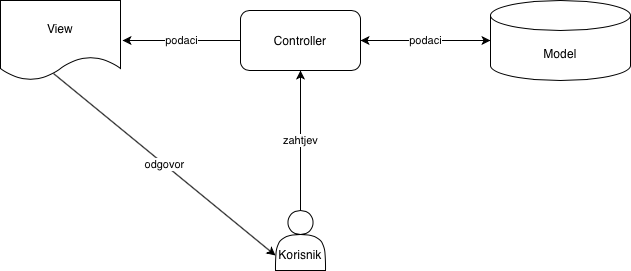
\includegraphics[scale=0.5]{slike/mvc.png}
			\caption{Arhitektura sustava}
		\end{figure}
	
		Praćenje MVC obrasca omogućuje razdvajanje ovisnosti i odgovornosti što rezultira u olakšanju paralelnog razvoja više dijelova aplikacije, testiranju i naknadnom dodavanju funkcionalnosti u sustav.
		
		Arhitektura sustava iz pogleda aktora sadrži sljedeće podsustave:
		
		\begin{packed_item}
			\item Aplikacija za sportaše i trenere
			\item Aplikacija za iznajmljivače
			\item Aplikacija za administratora
		\end{packed_item}
		
		Implementacijski je arhitektura podijeljena na backend i frontend.
		Frontend obuhvaća komponente vezane za vizualni prikaz kranjem korisniku i baziran je na \clickablefootnotelink{React-u}{https://reactjs.org/}, open-source Javascript biblioteci. Backend sloj izravno prati MVC razvojni obrazac i za njega je korišten programski jezik Java, točnije Spring okvir, kojemu je jedna od glavnih značajki inverzija ovisnosti. Osim toga nudi i gotove implementacije mnogobrojnih protokola i automatsko namještanje detaljnih postavki sustava. Za sigurnost je korišten JWT (JSON Web Token) koji je popularni otvoreni standard tokena za potpisivanje i enkripciju prilikom slanja podataka u JSON formatu.

				
		\section{Baza podataka}
			
		Kako bi se korisniku omogućila brza i efikasna izmjena i pregled podataka web aplikacija je u interakciji s bazom podataka. Baza zadovoljava treću normalnu formu te se brine o konzistentnosti podataka, primarnim i stranim ključevima te integritetskim ograničenjima. Baza se brine o istodobnom pristupu podacima, dakle transakcije zadovoljavaju svojstva ACID(Atomicity, Consistency, Isolation, Durability). Za upravljanje bazom podataka koristimo sustav PostgreSql zbog toga što je to besplatan sustav te je otvorenog koda i dostupan je za više operacijskih sustava.
		
			\subsection{Opis tablica}
			
			U nastavku navedeni su entiteti i atributi koje sadrži baza podataka te njihov tip podatka i opis. Atributi koji su u tablici označeni svijetlozelenom bojom predstavljaju primarni ključ, a atributi označeni svijetloplavom su strani ključevi.\\\\
				\begin{longtabu} to \textwidth {|X[6, l]|X[6, l]|X[20, l]|}
					\hline \multicolumn{3}{|c|}{\textbf{t\_user}}	 \\[3pt] \hline
					\endfirsthead
					\hline \multicolumn{3}{|c|}{\textbf{t\_user}}	 \\[3pt] \hline
					\endhead
					
					\hline 
					\endlastfoot
					
					\hline
					\cellcolor{LightGreen}id & INT	&  	Jedinstveni identifikator svakog korisnika registriranog u sustavu. 	\\ \hline
					username	 & VARCHAR & Korisničko ime s kojime se korisnik prijavljuje u sustav.  	\\ \hline 
					passwd\_hash & VARCHAR & Zaporka u obliku sažetka(hasha).  \\ \hline
				\end{longtabu}
				U relaciji t\_user nalaze se korisničko ime, zaporka te id koji služi kao jedinstveni identifikator svakog korisnika prijavljenog u sustav.
				
				
				\begin{longtabu} to \textwidth {|X[6, l]|X[6, l]|X[20, l]|}
					\hline \multicolumn{3}{|c|}{\textbf{t\_administrator}}	 \\[3pt] \hline
					\endfirsthead
					\hline \multicolumn{3}{|c|}{\textbf{t\_adminstrator}}	 \\[3pt] \hline
					\endhead
					
					\hline 
					\endlastfoot
					
					\hline
					\cellcolor{LightGreen}id & INT & Identifikator Jedinstveni identifikator svakog korisnika registriranog u sustav. \\ \hline
				\end{longtabu}
				Relacija t\_administrator sadrži identifikatore svih registriranih korisnika koji rade kao administratori sustava i imaju posebne ovlasti. Administrator odobrava i provjerava istinitost podataka i dokumenata koje prilažu iznajmljivači i treneri.  Id je strani ključ koji se poziva na relaciju t\_users. \\



				\begin{longtabu} to \textwidth {|X[6, l]|X[6, l]|X[20, l]|}
					\hline \multicolumn{3}{|c|}{\textbf{t\_person}}	 \\[3pt] \hline
					\endfirsthead
					\hline \multicolumn{3}{|c|}{\textbf{t\_person}}	 \\[3pt] \hline
					\endhead
					\hline 
					\endlastfoot
					\hline
					\cellcolor{LightGreen}id & INT	&  	Jedinstveni identifikator svakog korisnika registriranog u sustavu.\\ \hline
					email & VARCHAR & Email adresa sa kojom je povezan korisnički račun.  	\\ \hline
					name & VARCHAR & Korisnikovo ime.  	\\ \hline
					surname & VARCHAR & Korisnikovo prezime.  	\\ \hline 
					
				\end{longtabu}
				Relacija t\_person odnosi se na sve korisnike koji su registrirani kao sportaši, iznajmljivači ili treneri. Za njih bilježimo email ime i prezime. U relaciji tajođer postoji id kao strani ključ koji se poziva na relaciju t\_user. \\
				
				
				\begin{longtabu} to \textwidth {|X[6, l]|X[6, l]|X[20, l]|}
					\hline \multicolumn{3}{|c|}{\textbf{t\_athlete}}	 \\[3pt] \hline
					\endfirsthead
					\hline \multicolumn{3}{|c|}{\textbf{t\_person}}	 \\[3pt] \hline
					\endhead
					\hline 
					\endlastfoot
					\hline
					\cellcolor{LightGreen}id & INT	&  	Jedinstveni identifikator svakog korisnika registriranog u sustavu.\\ \hline
					birthday\_date\_date & TIMESTAMP & Datum rođernja sportaša.  	\\ \hline
					gender & VARCHAR & Spol sportaša.  	\\ \hline
					height & DOUBLE & Sportaševa visina izražena u cm.  	\\ \hline 
					weight & VARCHAR & Sportaševa težina izražena u kg.  \\ \hline
					
				\end{longtabu}
				Relacija t\_athlete sadrži sve bitne podatke o korisnicima koji se u sustav prijavljuju kao sportaši. Sportaši su korisnici koji se mogu prijaviti ili organizirazi sportska okupljanja odnosno događaje koji se ne naplaćuju i nisu pod profesionalnim vodstvom. U relaciji tajođer postoji id kao strani ključ koji se poziva na relaciju t\_users. \\
				
				
				\begin{longtabu} to \textwidth {|X[6, l]|X[6, l]|X[20, l]|}
					\hline \multicolumn{3}{|c|}{\textbf{t\_renter}}	 \\[3pt] \hline
					\endfirsthead
					\hline \multicolumn{3}{|c|}{\textbf{t\_renter}}	 \\[3pt] \hline
					\endhead
					\hline 
					\endlastfoot
					\hline
					\cellcolor{LightGreen}id & INT & Identifikator Jedinstveni identifikator svakog korisnika registriranog u sustav. \\ \hline
				\end{longtabu}
				Relacija t\_renter sadrži identifikatore svih registriranih korisnika koji su se u sustav prijavili kao iznajmljivači sportskih objekata. Oni u sustav mogu dodati svoj sportski objekt navodeći njegove specifikacije poput lokacije, tipa sportova koji se u tom objektu mogu igrati, cijene po satu i termine dostupne za rezervaciju. Id je strani ključ koji se poziva na relaciju t\_user. \\			
				
				
				
				
				\begin{longtabu} to \textwidth {|X[6, l]|X[6, l]|X[20, l]|}
					\hline \multicolumn{3}{|c|}{\textbf{t\_coach}}	 \\[3pt] \hline
					\endfirsthead
					\hline \multicolumn{3}{|c|}{\textbf{t\_coach}}	 \\[3pt] \hline
					\endhead
					\hline 
					\endlastfoot
					\hline
					\cellcolor{LightGreen}id & INT & Identifikator Jedinstveni identifikator svakog korisnika registriranog u sustav. \\ \hline
				\end{longtabu}
				Relacija t\_coach sadrži identifikatore svih trenera. Za razliku od sportaša treneri mogu organizirati i treninge  za koje mogu postaviti određenu cijenu. \\
				
				
				
				\begin{longtabu} to \textwidth {|X[6, l]|X[6, l]|X[20, l]|}
					\hline \multicolumn{3}{|c|}{\textbf{t\_location}}	 \\[3pt] \hline
					\endfirsthead
					\hline \multicolumn{3}{|c|}{\textbf{t\_location}}	 \\[3pt] \hline
					\endhead
					\hline 
					\endlastfoot
					\hline
					\cellcolor{LightGreen}id & INT & Jedinstveni identifikator svake lokacije dostupne u sustavu. \\ \hline
					 name & VARCHAR & Naziv lokacije.	\\ \hline
					 location\_type & VARCHAR &  Javna površina ili plaćeni sportski objekt.	\\ \hline
					 gpxcoordinates & VARCHAR & Geografske kordinate lokacije.	\\ \hline
					 \cellcolor{LightBlue}person\_id & INT & Identifikator korisnika koji je sportsku lokaciju dodao u sustav.\\
					 
				\end{longtabu}
				U relacijai t\_location nalaze sve sve lokacije unesene u sustav. Ovisno o tipu lokacije razlikujemo plaćene i javno dostupne lokacije. Za lokacije bilježi se id kreatora lokacije odnosno korisnika koji je unjeo u sustav lokaciju i potrebne podatke. Plaćene lokacije dopušteno je kreiraiti samo korisnicima kojima je odobren status iznajmljivača. Za plaćene lokacije evidentira se id iznajmljivača koji posjeduju taj objekt. Također u relaciji se spremaju kordinate lokacije koje mogu poslužiti kao marker na karti u slučaju jedne kordinate ili za iscrtavanje cijelog poligona u slučaju više zabilježenih koordinata.  \\
				
				
				
				\begin{longtabu} to \textwidth {|X[6, l]|X[6, l]|X[20, l]|}
					\hline \multicolumn{3}{|c|}{\textbf{t\_opening}}	 \\[3pt] \hline
					\endfirsthead
					\hline \multicolumn{3}{|c|}{\textbf{t\_opening}}	 \\[3pt] \hline
					\endhead
					\hline 
					\endlastfoot
					\hline
					\cellcolor{LightGreen}id & INT & Jedinstveni identifikator radnog vremena.	\\ 
					\hline
					cost & DOUBLE & Cijena u slučaju plaćene lokacije.	\\ \hline
					start\_time & TIME & Vrijeme otvaranja.	\\ \hline
					end\_time & TIME & Vrijeme zatvaranja.	\\ \hline
					from\_date & TIMESTAMP & Datum početka rasporeda.	\\ \hline
					to\_date & TIMESTAMP & Datum kraja rasporeda.	\\ \hline
					weekday & INT & Dan u tjednu na kojega se odnosi radno vrijeme.	\\ \hline
				\end{longtabu}
				Relacija t\_opening evidentiraju se radna vremena koja možemo pridružiti nkeim lokacijama. Za radno vrijeme evidentiraju se početak i kraj te u kojemu danu te datumi odkada dokada se takav raspred proteže. \\
				
				
				
				\begin{longtabu} to \textwidth {|X[6, l]|X[6, l]|X[20, l]|}
					\hline \multicolumn{3}{|c|}{\textbf{t\_location\_openings}}	 \\[3pt] \hline
					\endfirsthead
					\hline \multicolumn{3}{|c|}{\textbf{t\_location\_openings}}	 \\[3pt] \hline
					\endhead
					\hline 
					\endlastfoot
					\hline
					\cellcolor{LightGreen}paid\_location-\_id & INT & Identifikator lokacije za iznajmljivanje.	\\ \hline
					\cellcolor{LightGreen} openings\_id & INT & Identifikator radnog vremena iz realcije t\_opening.	\\ \hline
				\end{longtabu}
				Relacija t\_location\_open\_hours služi kao veza između relacija t\_opening i t\_location. U njoj su evidentirani radna vremena za sve plaćene lokacije.\\
				
				
				
				\begin{longtabu} to \textwidth {|X[6, l]|X[6, l]|X[20, l]|}
					\hline \multicolumn{3}{|c|}{\textbf{t\_sport}}	 \\[3pt] \hline
					\endfirsthead
					\hline \multicolumn{3}{|c|}{\textbf{t\_sport}}	 \\[3pt] \hline
					\endhead
					\hline 
					\endlastfoot
					\cellcolor{LightGreen}id & INT & Jedinstveni identifikator pojedinog sporta.	\\ \hline
					name & VARCHAR & Naziv sporta.	\\ \hline
					iconbwuri & VARCHAR & URI crno bijele ikone.	\\ \hline
					icon\_color\_uri & VARCHAR & URI ikone s bojom.	\\ \hline
					type & VARCHAR & Tip sporta (indoor/outdoor).	\\ \hline
				\end{longtabu}
				U relaciji t\_sport nalazi se popis svih sportova evidentiranih u sustavu. Svaki sport ima id, ime i tip u ovisnosti o tome igra li se sport u zatvorenom prostoru ili ne. \\
				
				
				\begin{longtabu} to \textwidth {|X[6, l]|X[6, l]|X[20, l]|}
					\hline \multicolumn{3}{|c|}{\textbf{t\_sportevent}}	 \\[3pt] \hline
					\endfirsthead
					\hline \multicolumn{3}{|c|}{\textbf{t\_sportevent}}	 \\[3pt] \hline
					\endhead
					\hline 
					\endlastfoot
					\cellcolor{LightGreen}id & INT & Jedinstveni identifikator svakog sportskog eventa.	\\ \hline
					\cellcolor{LightBlue} location\_id & INT & Jedinstveni identifikator lokacije na kojoj se održava sportski event.	\\ \hline
					\cellcolor{LightBlue} organizer\_id & INT & Jedinstveni identifikator organizatora sportskog eventa.	\\ \hline
					\cellcolor{LightBlue} sport\_id & INT & Jedinstveni identifikator sporta koji se igra na eventu.	\\ \hline
					sportevent-\_type & VARCHAR & Plaćeni ili neplaćeni event (amateur/professional).	\\ \hline
					max\_number-\_of\_participants & INT & Broj koliko ljudi maksimalno može sudjelovati na sportskom eventu.	\\ \hline
					start\_date\_time & TIMESTAMP & Datum i sat početka eventa.	\\ \hline
					end\_date\_time & TIMESTAMP & Datum i sat kraja eventa.	\\ \hline
					cost & DOUBLE & Cijena prisustvovanja u slučaju plaćenih eventova.	\\ \hline
					
				\end{longtabu}
				U relaciji t\_sportevent vidi se popis svih organiziranih sportskih eventova. Razlikujemo amaterskke i profesionalne eventove po tome plaćaju li se ili ne odnosno tko ih je organizirao trener ili sportaš. Za svaki event unesen u sustav poznat nam je datum i vrijeme početka i kraja eventa, maksimalan broj sudionika, cijena, koji sport se može igrati, tko je organizirao event i naravno na kojoj lokaciji će se event održavati.   \\
				
				
				
				\begin{longtabu} to \textwidth {|X[6, l]|X[6, l]|X[20, l]|}
					\hline \multicolumn{3}{|c|}{\textbf{t\_sportevent\_participants}}	 \\[3pt] \hline
					\endfirsthead
					\hline \multicolumn{3}{|c|}{\textbf{t\_sportevent\_participants}}	 \\[3pt] \hline
					\endhead
					\hline 
					\endlastfoot
					\cellcolor{LightGreen} events\_participation\_id & INT & Identifikator sportskog eventa u kojemu korisnik prisustvuje.	\\ \hline
					\cellcolor{LightGreen} participants\_id & INT & Identifikator korisnika koji prisustvuje u eventu.	\\ \hline
				\end{longtabu}
				U relaciji t\_sportevent\_participants evidentiramo id svakog korisnika koji prisustvuje u nekom eventu te id eventa u kojem prisustvuje.\\
				
				
				
				
				\begin{longtabu} to \textwidth {|X[6, l]|X[6, l]|X[20, l]|}
					\hline \multicolumn{3}{|c|}{\textbf{t\_documentation}}	 \\[3pt] \hline
					\endfirsthead
					\hline \multicolumn{3}{|c|}{\textbf{t\_documentation}}	 \\[3pt] \hline
					\endhead
					\hline 
					\endlastfoot
					
					\cellcolor{LightGreen}id & INT & Jedinstveni identifikator dokumenta.	\\ \hline
					document-\_intern\_uri & VARCHAR & Uri dokumenta.	\\ \hline
					type & INT & Vrsta dokumenta.	\\ \hline
					\cellcolor{LightBlue} approved\_by\_id & INT & Identifikator administratora koji je potvrdio dokument.	\\ \hline
				\end{longtabu}
				U relaciji t\_documentation nalazi se popis svih dokumenata koje prilažu sportaši koji žele postati treneri i iznajmljivači da bi im se priznao status iznajmljivača. Također evidentira se koji administrator potvrđuje ili odbacuje dokumentaciju. \\
				
				
				\begin{longtabu} to \textwidth {|X[6, l]|X[6, l]|X[20, l]|}
					\hline \multicolumn{3}{|c|}{\textbf{t\_coach\_coach\_certificate}}	 \\[3pt] \hline
					\endfirsthead
					\hline \multicolumn{3}{|c|}{\textbf{t\_coach\_coach\_certificate}}	 \\[3pt] \hline
					\endhead
					\hline 
					\endlastfoot
					
					\cellcolor{LightGreen}coach\_id & INT & Jedinstveni identifikator trenera.	\\ \hline
					\cellcolor{LightGreen} coach-\_certificate\_id & INT & Id dokumenta (certifikata trenera).	\\ \hline
				\end{longtabu}
				Relacija t\_coach\_coach\_certificate sadrži parove identifikatora trenera i identifikatora dokumenta koje prilažu da bi potvrdili svoj status trenera.  \\
				
				
				
				\begin{longtabu} to \textwidth {|X[6, l]|X[6, l]|X[20, l]|}
					\hline \multicolumn{3}{|c|}{\textbf{t\_location\_ownership\_certificate}}	 \\[3pt] \hline
					\endfirsthead
					\hline \multicolumn{3}{|c|}{\textbf{t\_location\_ownership\_certificate}}	 \\[3pt] \hline
					\endhead
					\hline 
					\endlastfoot
	
					\cellcolor{LightGreen}paid\_location-\_id & INT & Jedinstveni identifikator lokacije.	\\ \hline
					\cellcolor{LightGreen} ownership-\_certificate\_id & INT & Identifikator dokumenta.	\\ \hline
				\end{longtabu}
				Relacija t\_location\_ownership\_certificate sadrži parove identifikatora iznajmljivača i identifikatora dokumenta kojeg prilažu da bi dokazali da posjeduju sportski objekt kojeg žele iznajmljivati.  \\
				
				
				\begin{longtabu} to \textwidth {|X[6, l]|X[6, l]|X[20, l]|}
					\hline \multicolumn{3}{|c|}{\textbf{t\_documentation\_sports}}	 \\[3pt] \hline
					\endfirsthead
					\hline \multicolumn{3}{|c|}{\textbf{t\_documentation\_sports}}	 \\[3pt] \hline
					\endhead
					\hline 
					\endlastfoot
					
					\cellcolor{LightGreen}documentation-\_id & INT & Jedinstveni identifikator dokumenta.	\\ \hline
					\cellcolor{LightGreen} sports\_id & INT & Identifikator sporta.	\\ \hline
				\end{longtabu}
				Relacija t\_documentation\_sports sadrži parove identifikatora dokumenta koje trener prilaže da mu se potvrdi status trenera i identifikatora sporta na koji se taj dokument odnosi.  \\
				
				
				
				\begin{longtabu} to \textwidth {|X[6, l]|X[6, l]|X[20, l]|}
					\hline \multicolumn{3}{|c|}{\textbf{t\_location\_available\_sports}}	 \\[3pt] \hline
					\endfirsthead
					\hline \multicolumn{3}{|c|}{\textbf{t\_location\_available\_sports}}	 \\[3pt] \hline
					\endhead
					\hline 
					\endlastfoot
					
					\cellcolor{LightGreen} location\_id & INT & Jedinstveni identifikator lokacije.	\\ \hline
					\cellcolor{LightGreen} available-\_sports\_id & INT & Identifikator sporta.	\\ \hline
				\end{longtabu}
				Relacija t\_location\_available\_sports sadrži parove identifikatora lokacije i sportova koji se mogu igrati na toj lokaciji.  \\
				
				
				\begin{longtabu} to \textwidth {|X[6, l]|X[6, l]|X[20, l]|}
					\hline \multicolumn{3}{|c|}{\textbf{t\_sportevent\_location\_reservation\_inquery}}	 \\[3pt] \hline
					\endfirsthead
					\hline \multicolumn{3}{|c|}{\textbf{t\_sportevent\_location\_reservation\_inquery}}	 \\[3pt] \hline
					\endhead
					\hline 
					\endlastfoot
					
					\cellcolor{LightGreen} reservation-\_queue\_id & INT & Jedinstveni identifikator liste za čekanje.	\\ \hline
					\cellcolor{LightGreen} location-\_reservation-\_inquery\_id & INT & Identifikator rezervacije.	\\ \hline
				\end{longtabu}
				Relacija t\_sportevent\_location\_reservation\_inquery Sadrži podatke o rezervaciji lokacije za sportska događanja.  \\
				
				
				
				
				

	
			
		\newgeometry{left=0.5cm,bottom=0.5cm,right=0.5cm,top=0.5cm}
		\begin{landscape}
			
			\section{Dijagram baze podataka}
			\thispagestyle{empty}
			\begin{figure}[ht!]
				\centering
				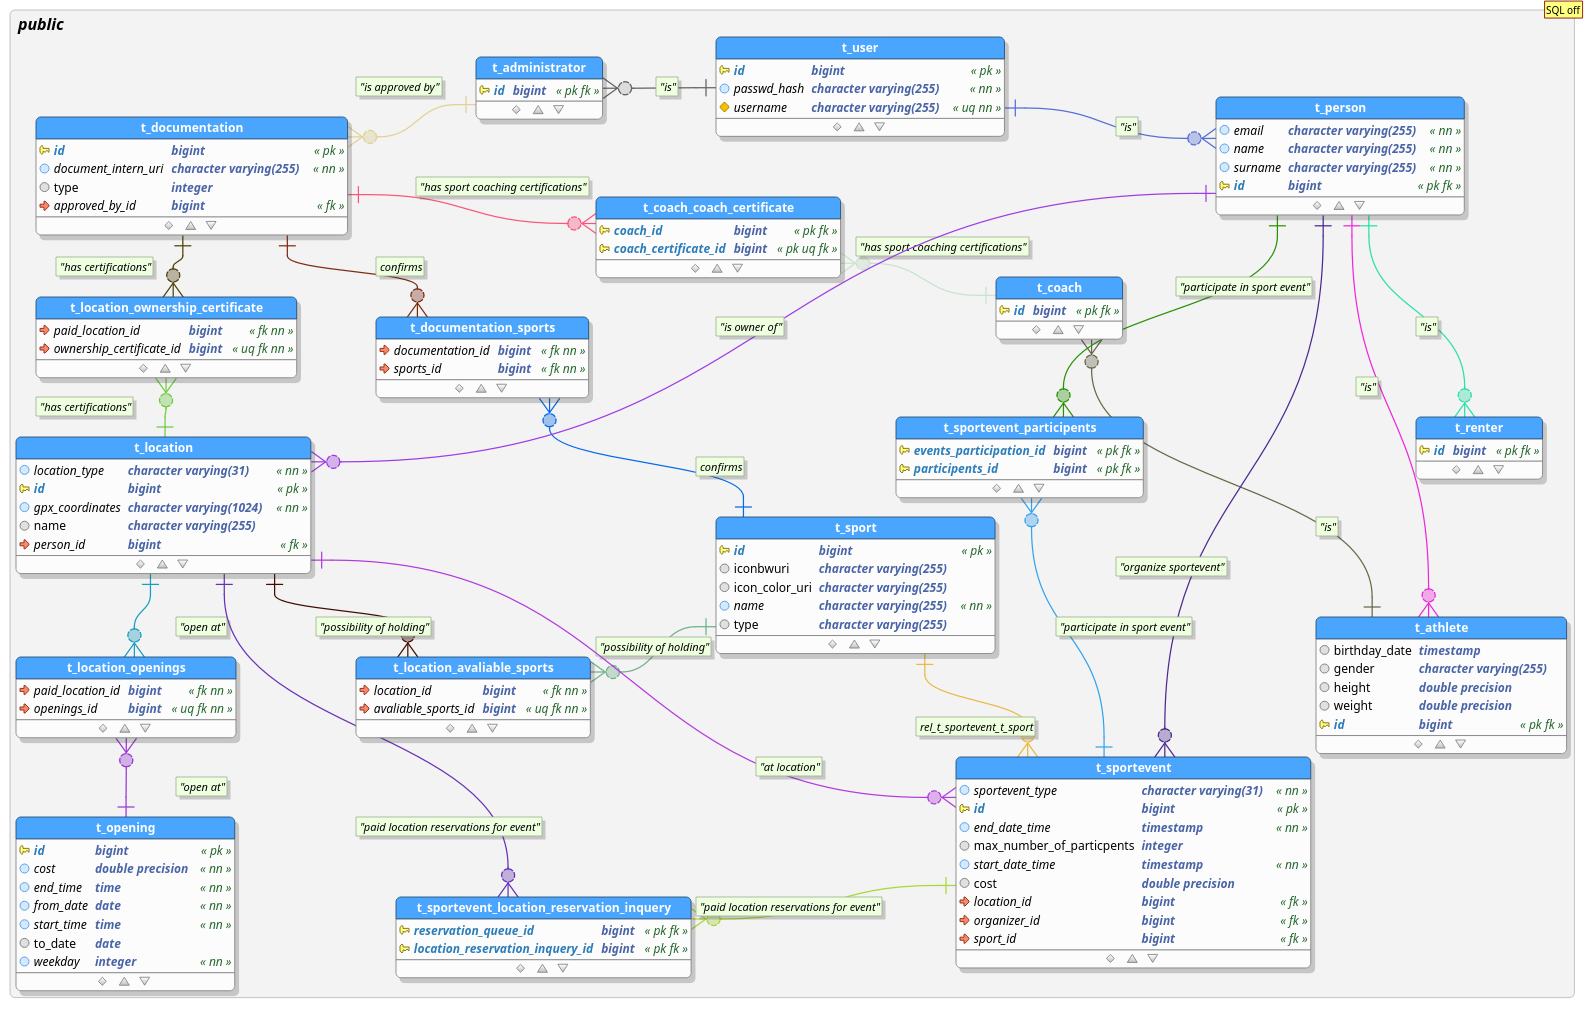
\includegraphics[scale=0.60]{slike/bazapodataka.png}
				\caption{Dijagram baze podataka}
			\end{figure}
			
		\end{landscape}
		\restoregeometry
			
			\eject
		\newgeometry{left=0.5cm,bottom=0.5cm,right=0.5cm,top=0.5cm}
		\begin{landscape}
		
			\section{Dijagram razreda}
			\thispagestyle{empty}
			\begin{figure}[ht!]
				\centering
				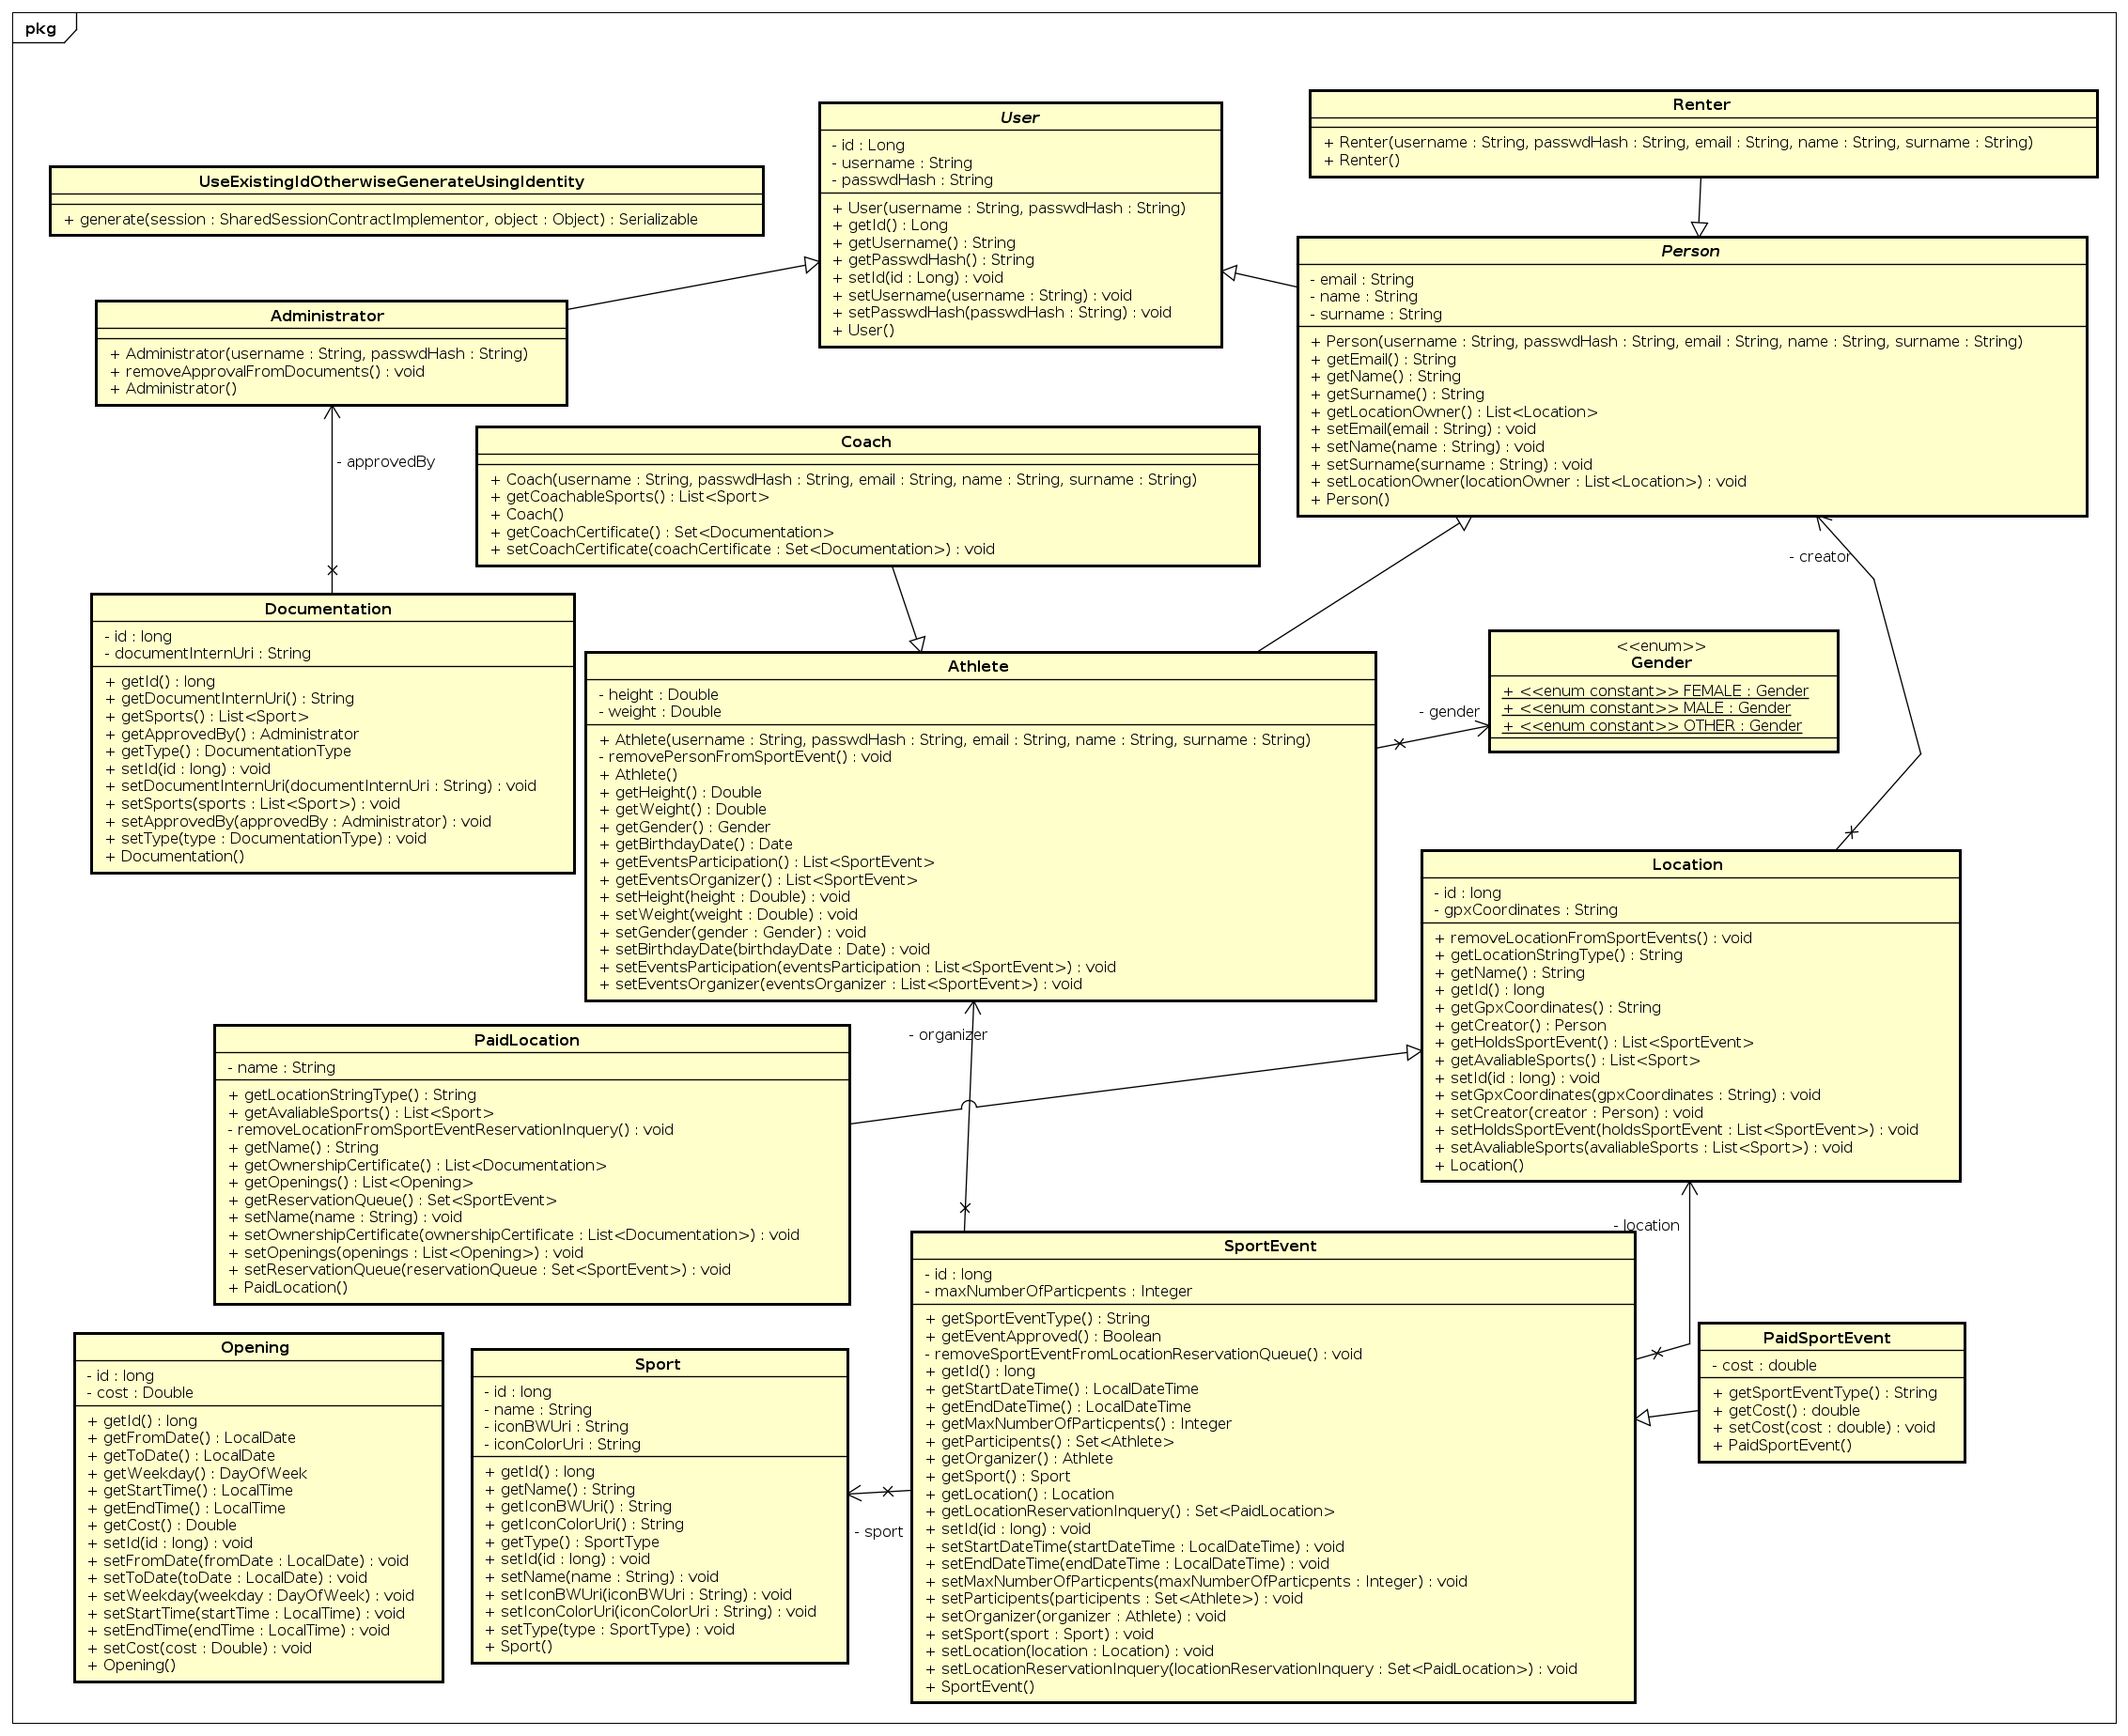
\includegraphics[scale=0.35]{dijagrami/dijagram_razreda_domena.png}
				\caption{Dijagram razreda}
			\end{figure}
			
		\end{landscape}
		\restoregeometry
		\eject
		
		Razred \textbf{User} predstavlja registriranog korisnika koji sadrži atribute username i password. Različite vrste korisnika reprezentiramo razredima Administrator, Person, Athlete, Coach, Renter.\\
		Razred \textbf{Person} nasljeđuje User i predstavlja fizičku osobu te sadrži osobne podatke. \textbf{Athlete} nasljeđuje razred Person i predstavlja sportaša, dok \textbf{Coach} nasljeđuje razred Athlete.\\
		Razred \textbf{Coach} sadrži i referencu na svoju dokumentaciju koja potvrđuje da je službeni trener za određene sportove.\\
		Razred \textbf{Renter} predstavlja iznajmljivača i nasljeđuje razred Person. Razred \textbf{Administrator} nasljeđuje razred User te sadrži referencu na sve dokumente (\textbf{Documentation}) koje je potvrdio.\\
		Razred \textbf{Location} predstavlja lokaciju nekog sportskog okupljanja kojeg je kreirao sportaš, te sadrži atribut GPXCoordinates u kojem su zapisane GPX koordinate objekta. Lokacija sadrži referencu na osobu (Person) koja ju je napravila.\\
		Razred \textbf{PaidLocation} predstavlja lokaciju koju je iznajmljuje iznajmljivač (\textbf{Renter}). Plaćena lokacija sadrži popis radnih sati (\textbf{Opening}) i popis sportova (\textbf{Sport}) koji se mogu igrati na navedenoj lokaciji. Također lokacija koja se iznajmljuje mora imati dokumentaciju o objektu (\textbf{Documentation}) koju potvrđuje Administrator.\\
		Razred \textbf{Opening} predstavlja jedan segment radnog vremena. Segment je definiran danom u tjednu (\textbf{weekday}) i početnim (\textbf{start\_time}) i završnim satom (\textbf{end\_time}). Takav segment se ponavlja sve dok je unutar područja aktivnosti definiranog s početnim datumom (\textbf{from\_date}) i završnim datumom (\textbf{to\_date}).\\
		Razred \textbf{SportEvent} predstavlja događaj koje ovisno o tipu može biti sportsko okupljanje ili profesionalni trening. SportEvent sadrži referencu na lokaciju događaja (\textbf{Location}) i na osobu koja je napravila događaj (\text{Athlete}). Ako događaj iznajmljuje objekt (\textbf{PaidLocation}) tada iznajmljivač putem atributa location\_approved potvrđuje rezervaciju objekta.\\
		Razred \textbf{Documentation} predstavlja dokumentaciju te sadrži interni url PDF datoteke koja je prenesena. Također sadrži i referencu na sportove koji se odnose na dokumentaciju. Dokumentaciju potvrđuje administrator. Razred \textbf{Sport} sadrži informacije vezane uz jedan sport. 
		\eject
		
		\newgeometry{left=2.0cm,bottom=0.5cm,right=0.5cm,top=0.5cm}
		\begin{landscape}
			\thispagestyle{empty}

			\begin{figure}[ht!]
				\centering
				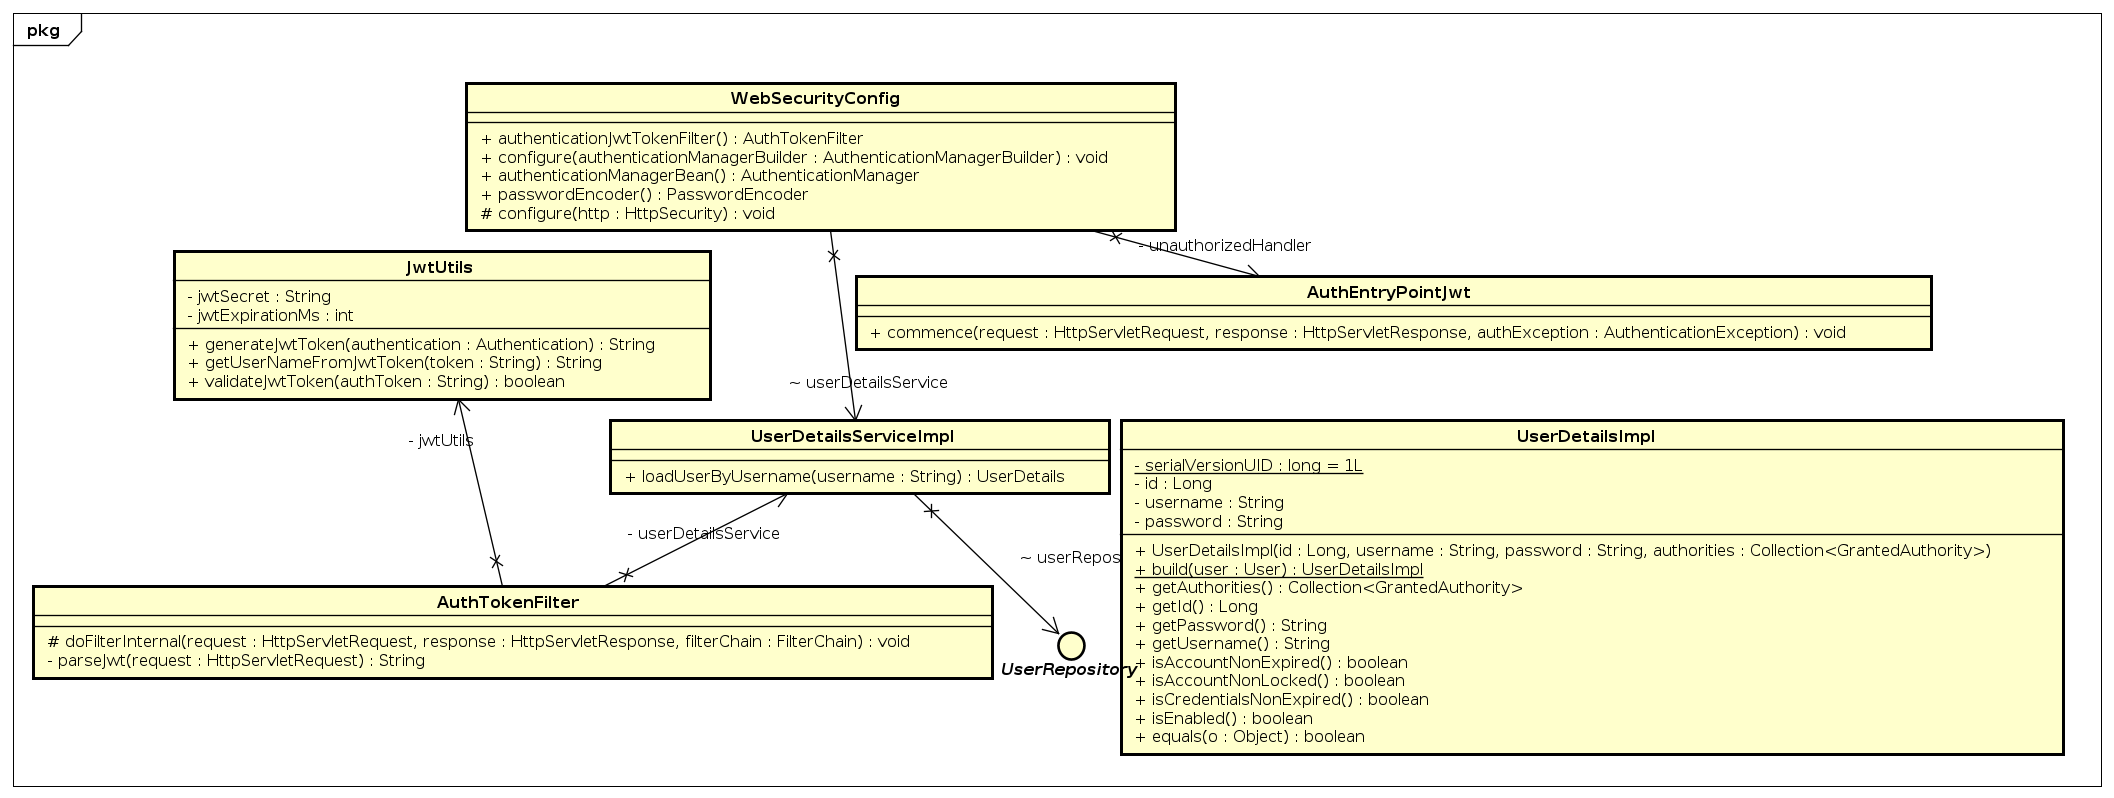
\includegraphics[scale=0.50]{dijagrami/dijagram_razreda_JWT_security.png}
				\caption{Dijagram razreda JWT autentifikacije}
			\end{figure}
			
		\end{landscape}
		\restoregeometry
		\eject
		
		U razredu \textbf{WebSecurityConfig} koji implementira WebSecurityConfigurerAdapter sučelje postavljamo opcije vezane uz Spring Security. Razred \textbf{AuthEntryPointJwt} implementira AuthenticationEntryPoint te se metoda commence pokreće svaki put kada neregistrirani korisnik pristupi zaštićenom sadržaju, te se vraća HTTP 401 UNAUTHORIZED. Kako bi Spring Security omogućili da učita korisnika implementiramo sučelje UserDetailsService u razredu \textbf{UserDetailsServiceImpl}, a podatke samog korisnika spremamo u razredu \textbf{UserDetailsImpl}. Razred \textbf{JwtUtils} pruža metode za parsiranje, generiranje, i validaciju JWT.
		
		\begin{figure}[H]
			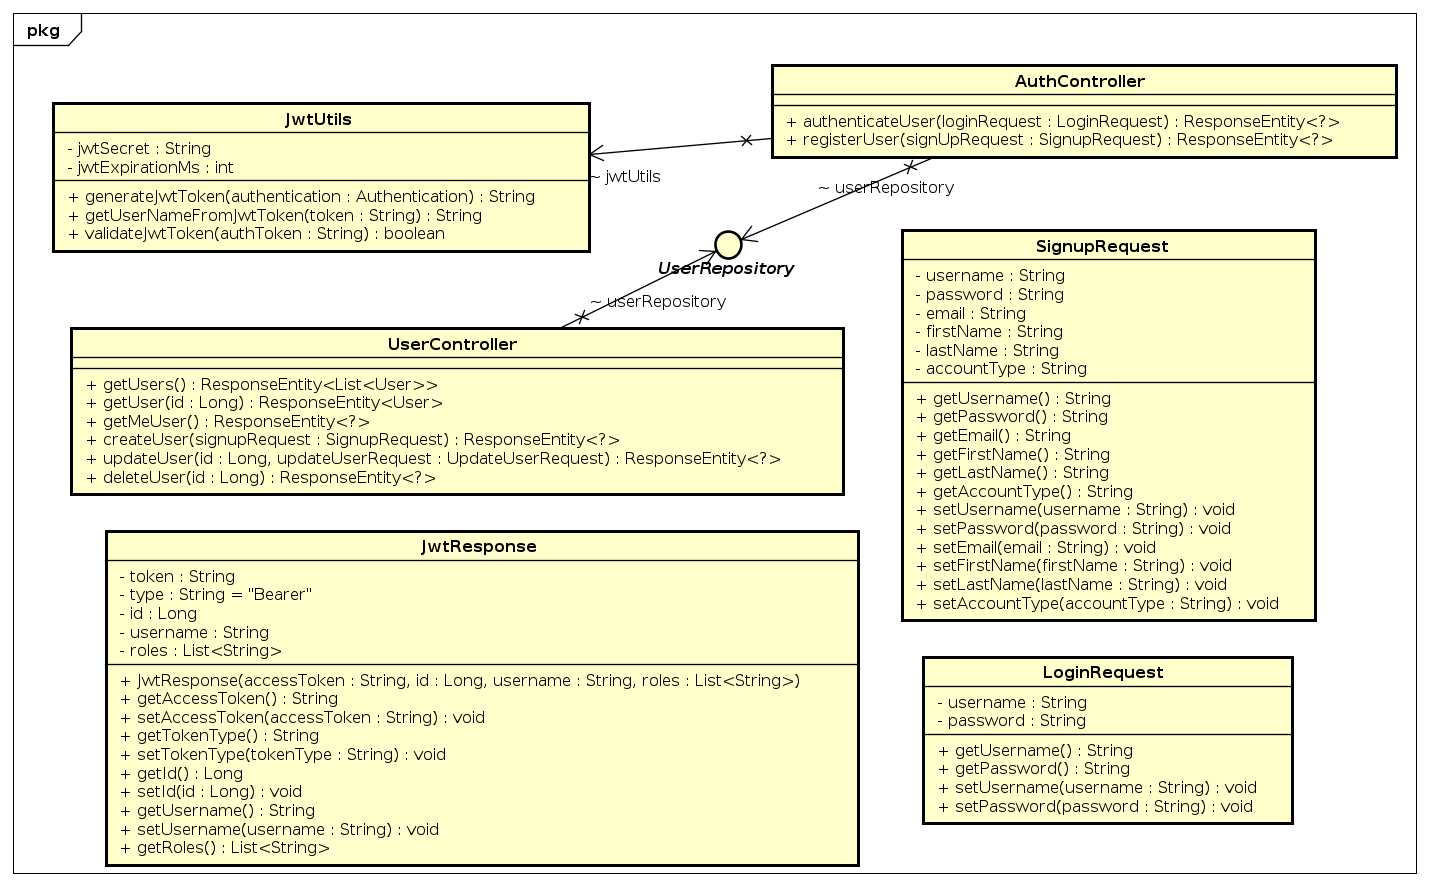
\includegraphics[width=\textwidth]{dijagrami/dijagram_razreda_login.png}
			\caption{Dijagram razreda prijave u sustav}
		\end{figure}
	
		Razred \textbf{AuthController} poslužuje zahtjeve za prijavu i registraciju koje prima pomoću razreda \textbf{LoginRequest} i \textbf{SignupRequest}. Dok razred \textbf{ProfileController} poslužuje osnovne informacije o prijavljenom korisniku.
		
		
		\begin{figure}[H]
			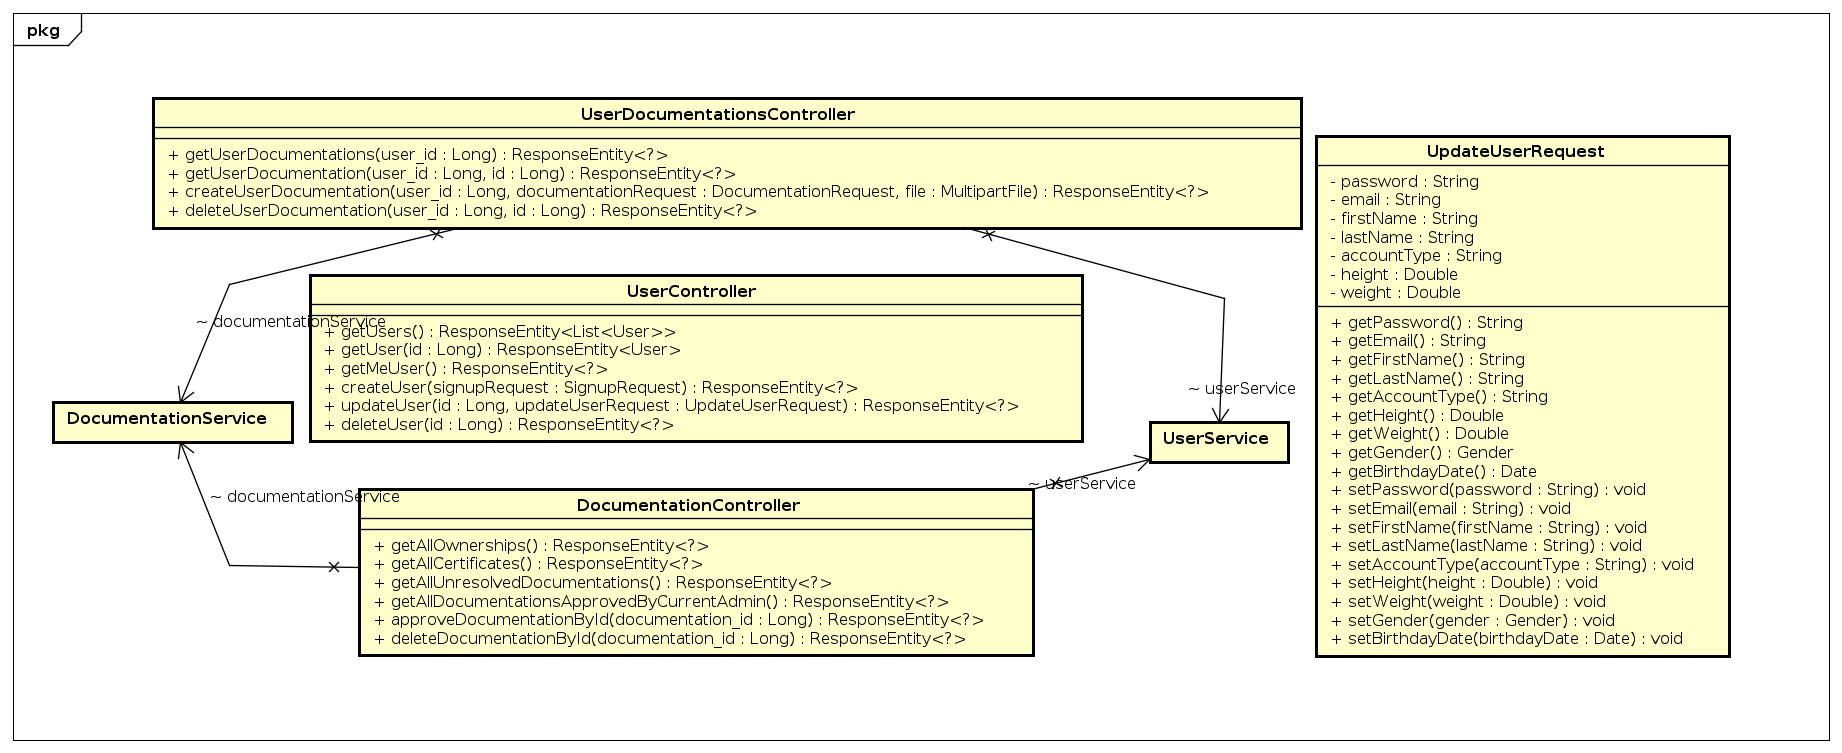
\includegraphics[width=\textwidth]{dijagrami/dijagram_razreda_user.png}
			\caption{Dijagram razreda osnovnih korisničkih funkcionalnosti}
		\end{figure}
		Razred \textbf{UserController} omogućuje pregled osnovnih informacija o korisniku. Također pomoću podataka koje prima preko razreda \textbf{UpdateUserRequest} može vršiti osvježavanje podataka korisnika. Razred \textbf{UserDocumentationController} poslužuje zahtjeve za predaju dokumentacija trenera. Razred \textbf{DocumentationController} služi za pregled dokumentacija trenera i lokacija od strane administratora te povrđivanje ili uklanjanje. 
		
	
	
		\begin{figure}[H]
			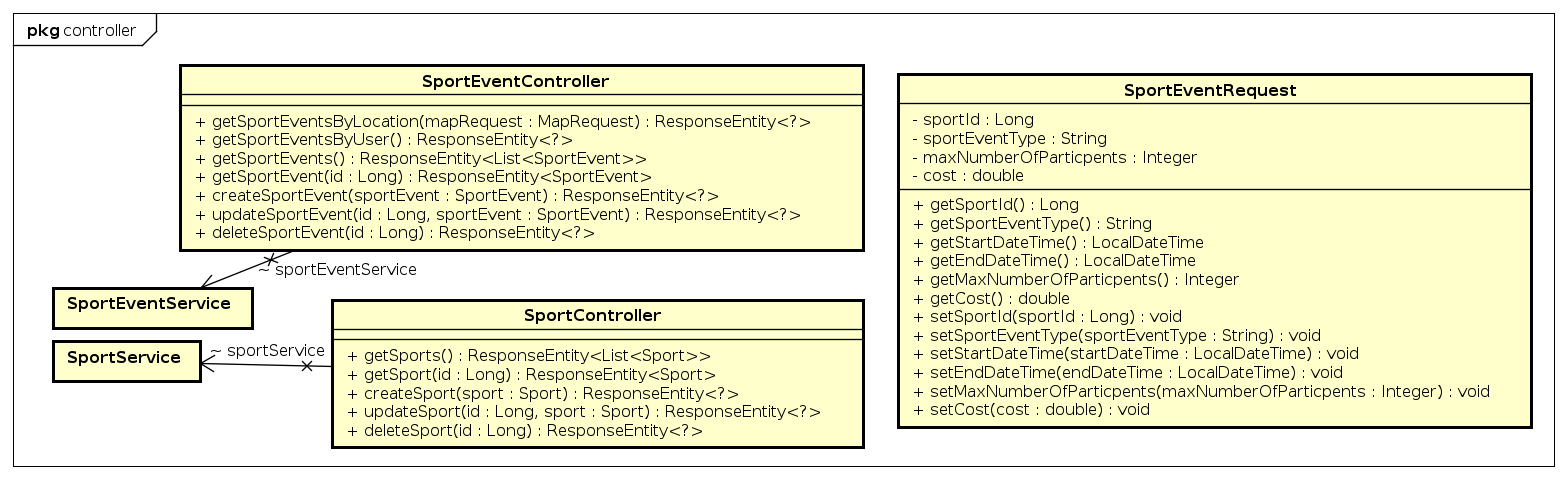
\includegraphics[width=\textwidth]{dijagrami/dijagram_razreda_sportevente.png}
			\caption{Dijagram razreda funkcionalnosti sportskih okupljanja}
		\end{figure}
	
		Razred \textbf{SportEventController} poslužuje osnovne informacije o sportskim okupljanjima. Također omogućuje dobivanje podataka o sportskim okupljanjima na nekoj lokaciji. Razred \textbf{SportController} služi za dohvaćanje podataka o sportovima koji su dostupni unutar aplikacije.
	
	
		\newgeometry{left=2.0cm,bottom=0.5cm,right=0.5cm,top=0.5cm}
		\begin{landscape}
			\thispagestyle{empty}
			
			\begin{figure}[ht!]
				\centering
				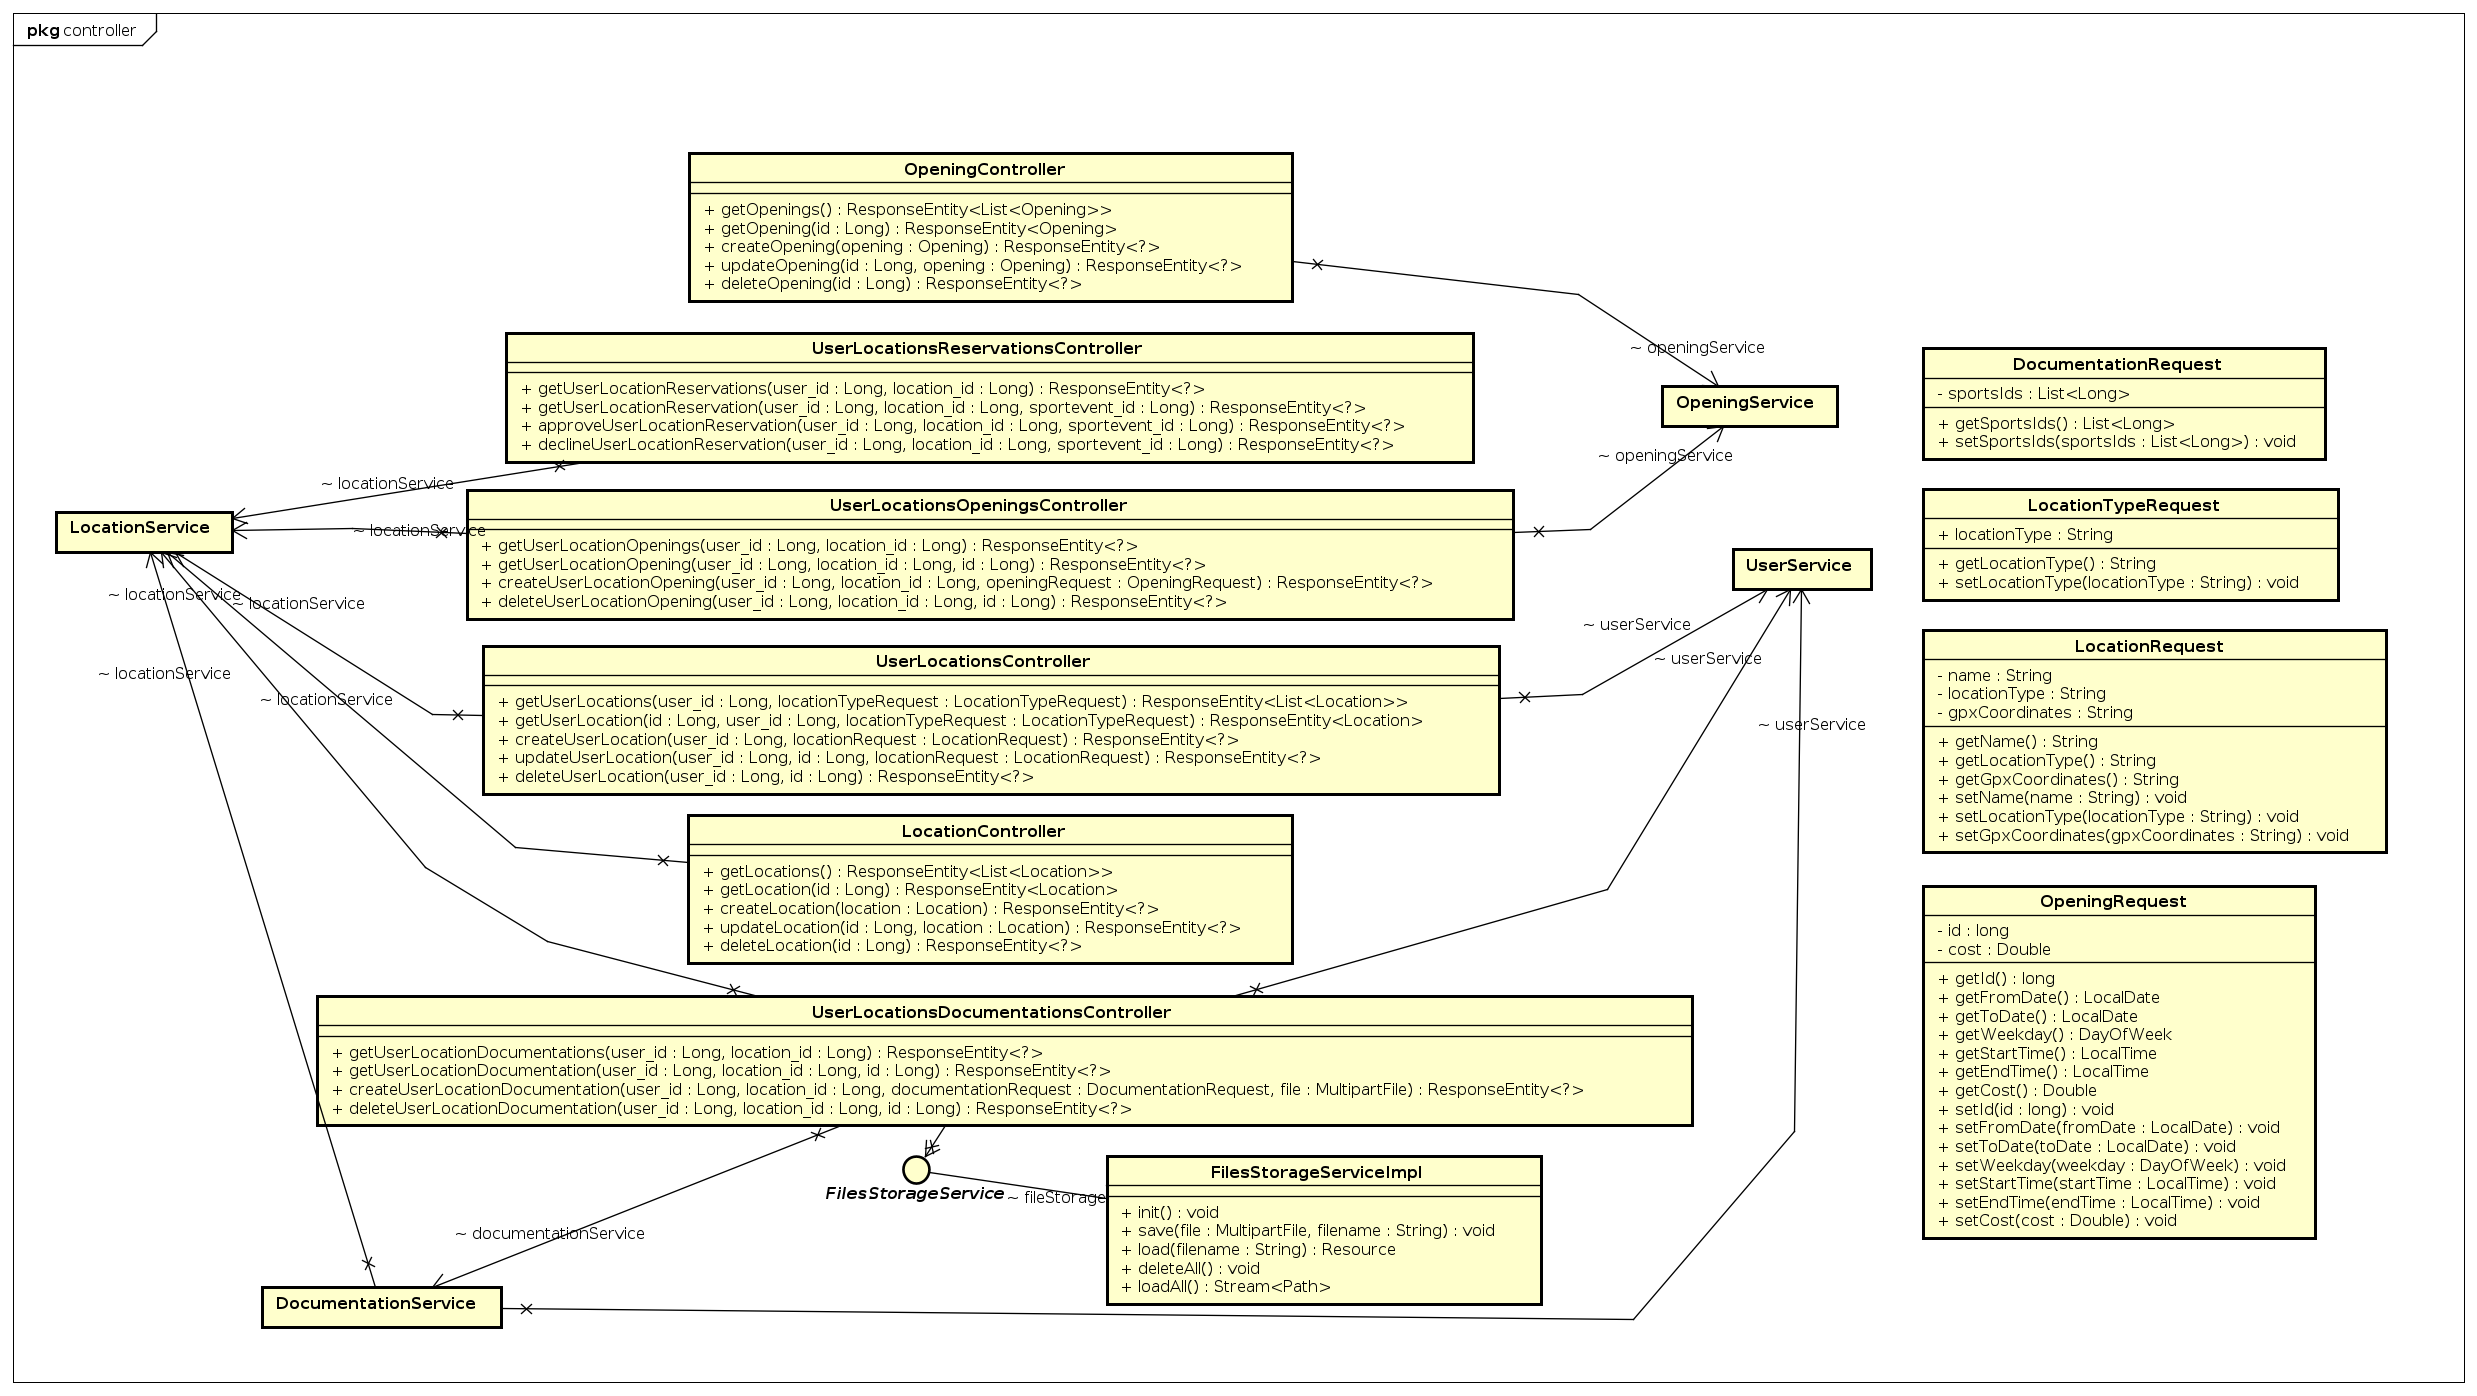
\includegraphics[scale=0.40]{dijagrami/dijagram_razreda_za_lokacije.png}
				\caption{Dijagram razreda funkcionalnost lokacija}
			\end{figure}
			
		\end{landscape}
		\restoregeometry
		\eject
	
		\newgeometry{left=2.0cm,bottom=0.5cm,right=0.5cm,top=0.5cm}
		\begin{landscape}
			\thispagestyle{empty}
			
			\begin{figure}[ht!]
				\centering
				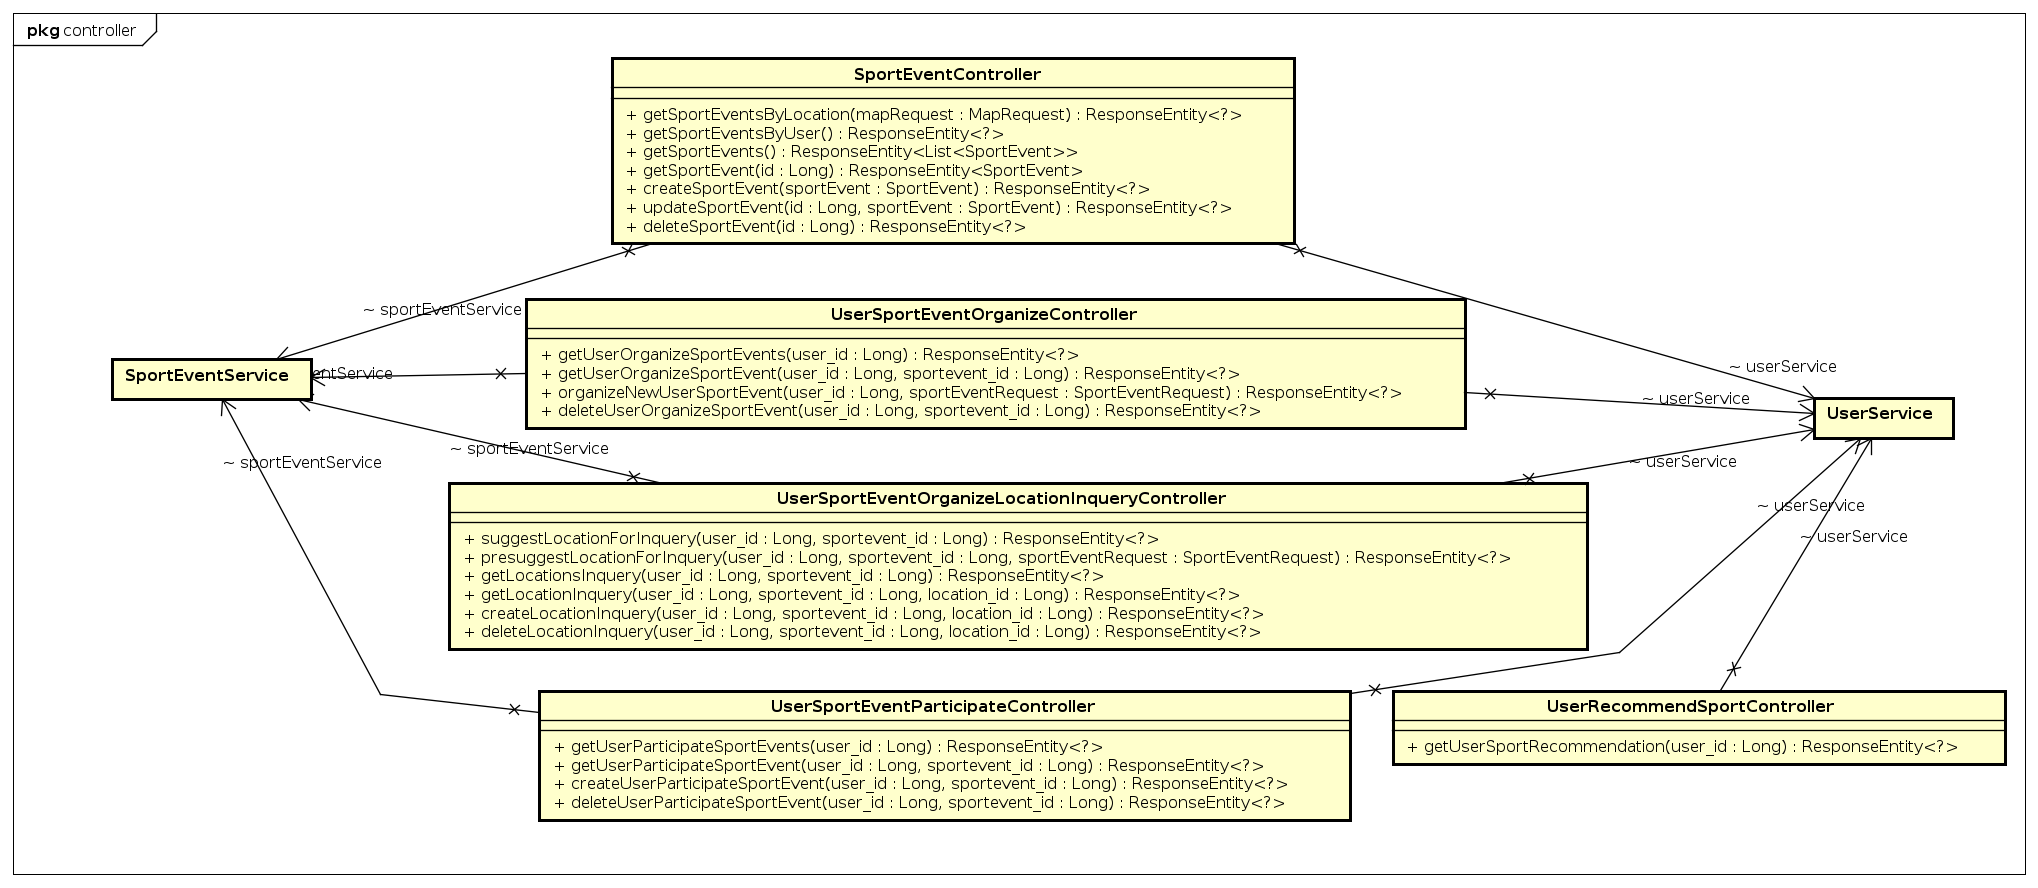
\includegraphics[scale=0.50]{dijagrami/dijagram_razreda_sportevent_lokacije.png}
				\caption{Dijagram razreda veze lokacija i sportskih okupljanja}
			\end{figure}
			
		\end{landscape}
		\restoregeometry
		\eject
	
		Razred \textbf{OpeningController} poslužuje informacije o radnom vremenu lokacije. Razred \textbf{LocationController} omogućuje pregled lokacija. Razred \textbf{UserLocationController} služi za upravljanje korisnikovih lokacija. \textbf{UserLocationsOpenings} omogućuje postavljanje radnog vremena korisnikovoj lokaciji koja se plaća. Razred \textbf{UserLocationsReservationsController} omogućuje potvrđivanje rezervacije nekog sportskog okupljanja na pojedinoj lokaciji. Razred \textbf{UserLocationsDocumentationsController} omogućuje iznajmljivačima prijenos dokumentacija na poslužitelj.
		\hfill\break
		
		Razred \textbf{UserSportEventOrganizeController} omogućuje sportašu slanje zahtjeva za organiziranje sportskih okupljanja. Svako sportsko okupljanje može zatražiti rezervaciju plaćene lokacije preko razreda \textbf{UserSportEventOrganizeLocationInqueryController}. Sportaš preko razreda \textbf{UserSportEventParticipateController} se može prijaviti na sportsko okupljanje.
	
%			\textit{Potrebno je priložiti dijagram razreda s pripadajućim opisom. Zbog preglednosti je moguće dijagram razlomiti na više njih, ali moraju biti grupirani prema sličnim razinama apstrakcije i srodnim funkcionalnostima.}\\
			
%			\textbf{\textit{dio 1. revizije}}\\
			
%			\textit{Prilikom prve predaje projekta, potrebno je priložiti potpuno razrađen dijagram razreda vezan uz \textbf{generičku funkcionalnost} sustava. Ostale funkcionalnosti trebaju biti idejno razrađene u dijagramu sa sljedećim komponentama: nazivi razreda, nazivi metoda i vrste pristupa metodama (npr. javni, zaštićeni), nazivi atributa razreda, veze i odnosi između razreda.}\\
%			
%			\textbf{\textit{dio 2. revizije}}\\			
%			
%			\textit{Prilikom druge predaje projekta dijagram razreda i opisi moraju odgovarati stvarnom stanju implementacije}
			
			
			
			\eject
		
		\section{Dijagram stanja}
			Na slici 4.7 je prikazan dijagram stanja za iznajmljivanje prostora za sport. Korisnik s početne stranice "Naslovnica" klikom na "Iznajmi prostor za sport" dolazi na stranicu za iznajmljivanje prostora za sport. Na toj stranici korisnik može pregledati dostupne prostore za sport, nakon odabira prostora, korisnik odabire dostupan datum i vrijeme termina. Prije klika na "Potvrdi rezervaciju" korisnik može odustati od rezervacije klikom na "Odustani" i vratiti se nazad na stranicu za pregled dostupnih prostora za sport. Nakon odabira prostora, datuma i termina korisnik završava rezervaciju klikom na "Potvrdi rezervaciju" te čeka potvrdu rezervacije. Nakon što sustav potvrdi rezervaciju korisnik bira hoće li napraviti još rezervacija ili ne, ako odabere da želi napraviti još rezervacija sustav ga vrati na stranicu za iznajmljivanje prostora za sport, inače ga vrati na "Naslovnicu". Ako dođe do greške prilikom rezervacije sustav obavijesti korisnika o greški te ga vrati na početnu stranicu za iznajmljivanje. Korisnik se može s početne stranice za iznajmljivanje vratiti na "Naslovnicu" klikom na "Povratak na Naslovnicu".
			
			\begin{figure}[H]
				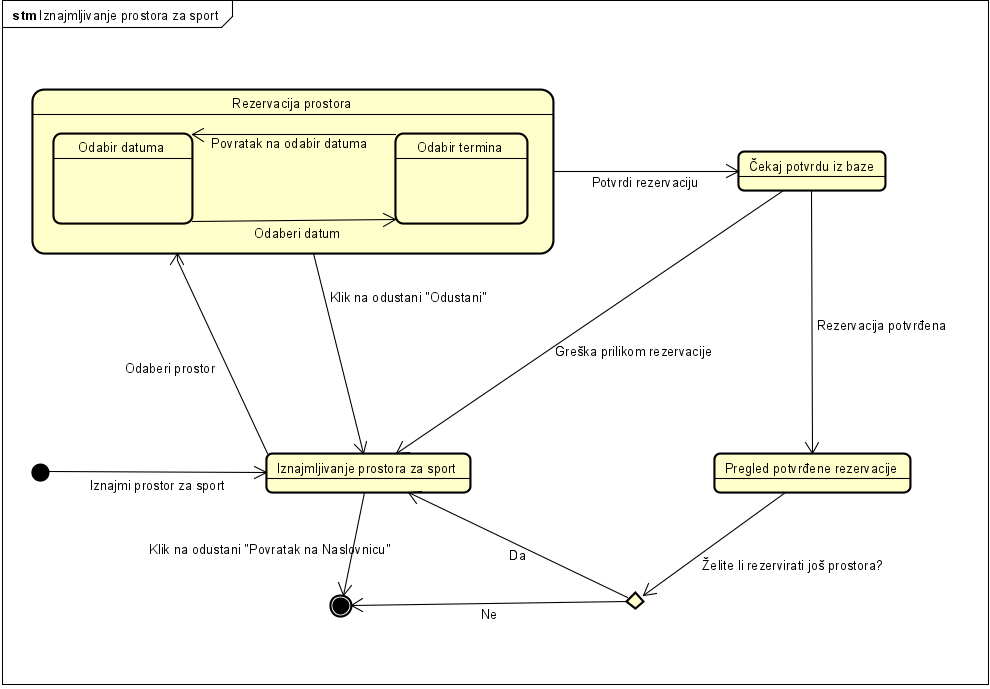
\includegraphics[width=\textwidth]{slike/dijagramStanja.png}
				\caption{Dijagram stanja iznajmljivanja prostora za sport}
			\end{figure}
%			\textbf{\textit{dio 2. revizije}}\\
			
%			\textit{Potrebno je priložiti dijagram stanja i opisati ga. Dovoljan je jedan dijagram stanja koji prikazuje \textbf{značajan dio funkcionalnosti} sustava. Na primjer, stanja korisničkog sučelja i tijek korištenja neke ključne funkcionalnosti jesu značajan dio sustava, a registracija i prijava nisu. }
			
			
			\eject 
		
		\section{Dijagram aktivnosti}
			Na slici 4.8 prikazan je dijagram aktivnosti predaje dokumentacije trenera i prikaz aktivnosti potvrđivanja (ili odbijanja) predane dokumentacije. Trener preda dokumentaciju aplikaciji te aplikacija tu dokumentaciju spremi u bazu. Prilikom spremanja dokumentacije u bazu se zapisuje i podatak da je ta dokumentacija nepotvrđena. Administrator može zatražiti od aplikacije popis svih nepotvrđenih dokumentacija, aplikacija ih uzme iz baze te prikaže administratoru. Administrator pregledava dokumentacije te odlučuje hoće li ih odbaciti (izbrisati) ili potvrditi. Nakon što administrator donese odluku o dokumentaciji trener dobiva obavijest o odluci admnistratora.
			
			\begin{figure}[H]
				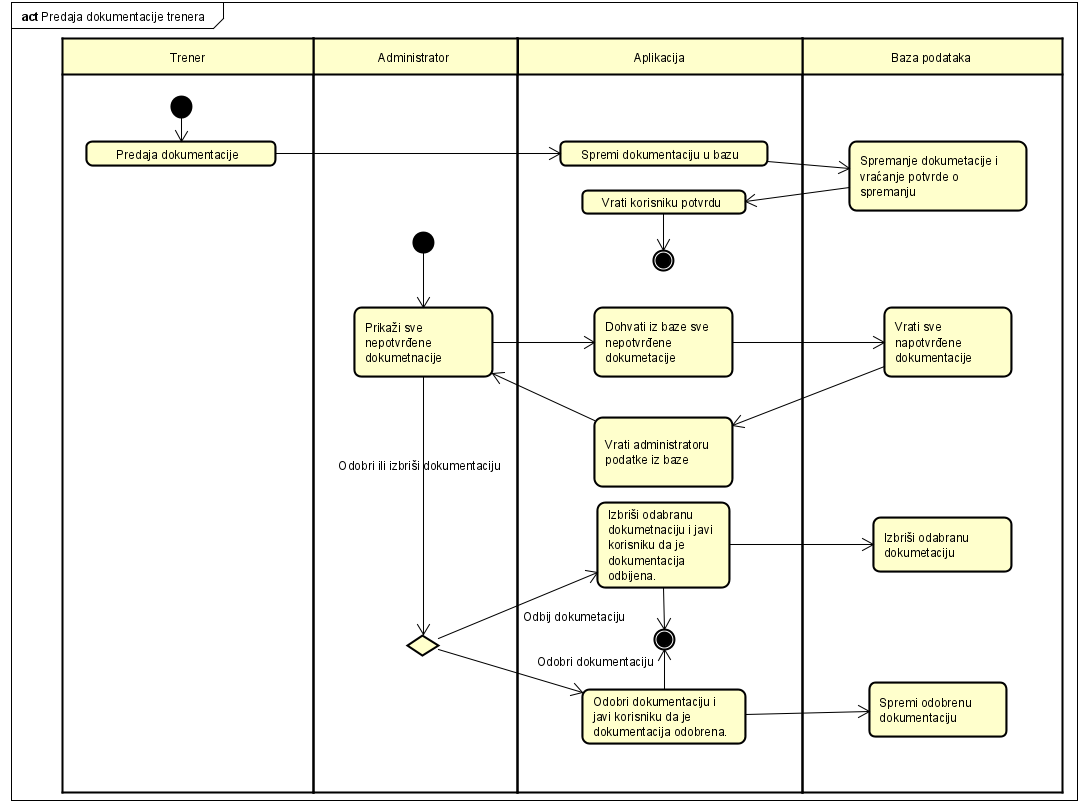
\includegraphics[width=\textwidth]{slike/dijagramAktivnosti.png}
				\caption{Dijagram aktivnosti predaje dokumentacije za trenera}
			\end{figure}
%			\textbf{\textit{dio 2. revizije}}\\
%			
%			 \textit{Potrebno je priložiti dijagram aktivnosti s pripadajućim opisom. Dijagram aktivnosti treba prikazivati značajan dio sustava.}
%			
			\eject
		\section{Dijagram komponenti}
			Dijagram komponenti prikazan na slici opisuje organizaciju i međuovisnost komponenti aplikacije. Aplikaciji se pristupa s web preglednika kojem React biblioteka poslužuje HTML, CSS i Javascript datoteke generirane iz Javascript datoteka predanih biblioteci. React aplikacija odnosno "frontend" dio web aplikacije s "backend" dijelom komunicira slanjem podataka u JSON formatu pomoću programskog paketa Axios. Za osjetljive podatke poput korisničkih informacija podaci se šalju u obliku JWT, odnosno JSON Web Token."Backend" dio web aplikacije s bazom podataka komunicira preko komponente Repository, a podaci dobiveni iz baze podataka koriste se dalje u "backend" dijelu  web aplikacije. "Backend" dio web aplikacije također komunicira s predikcijom sporta strojnim učenjem.
			
			\begin{figure}[H]
				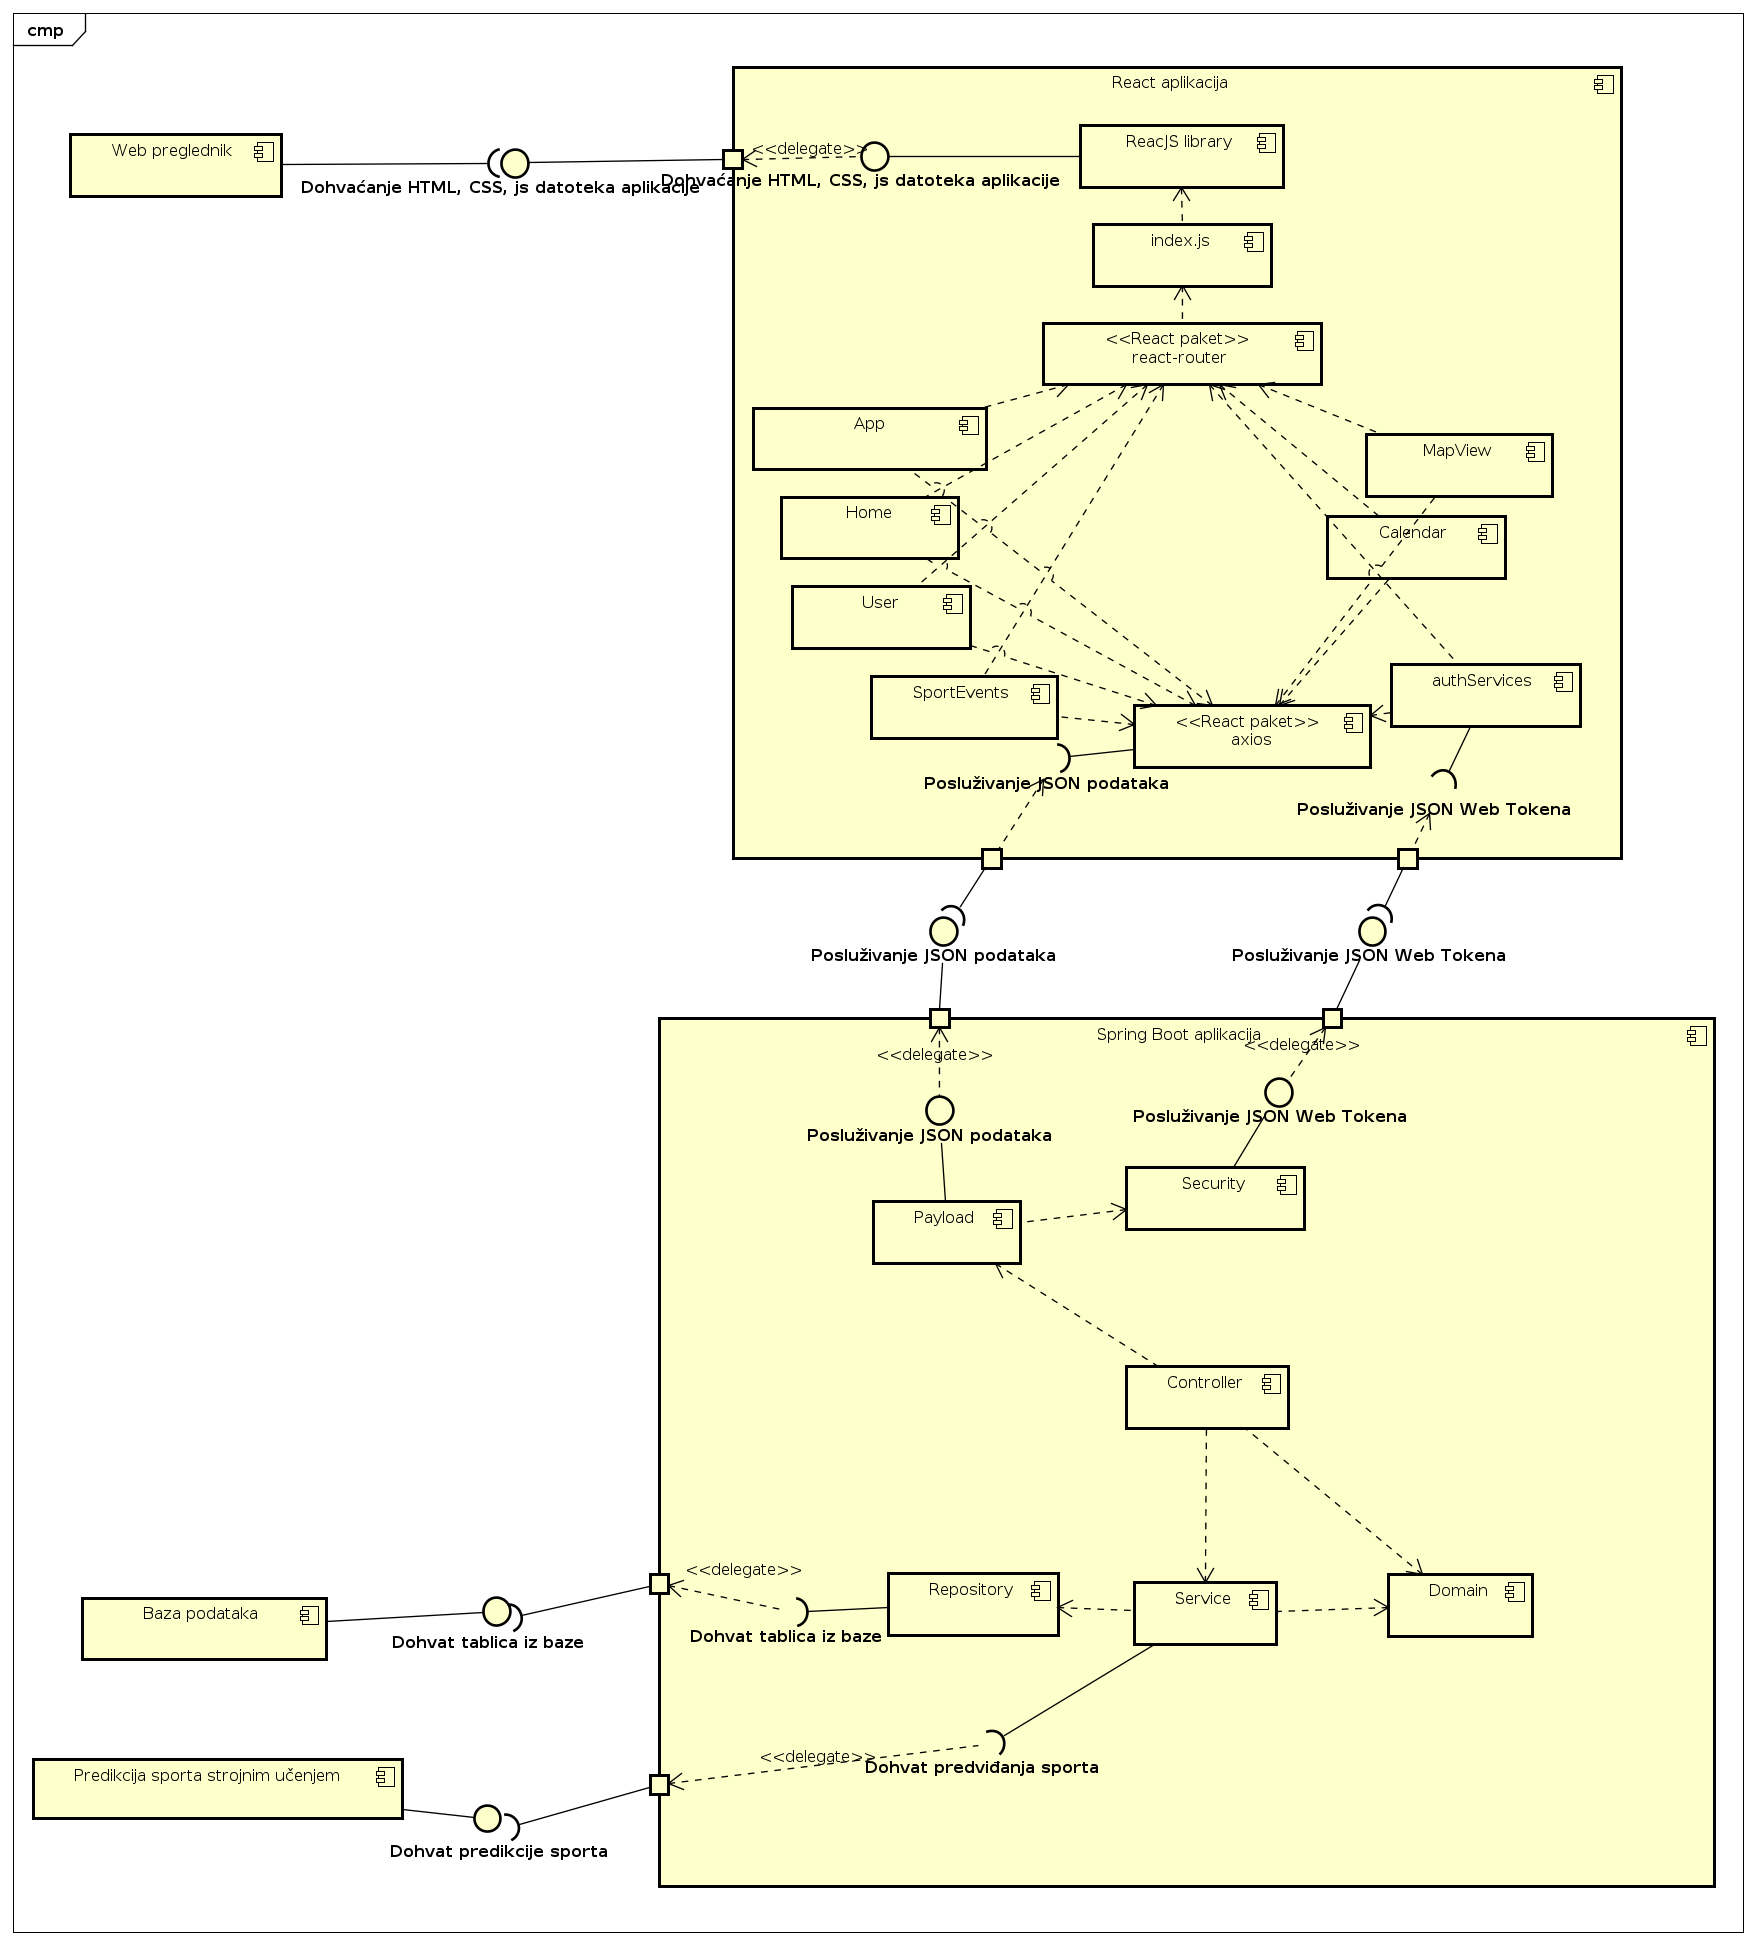
\includegraphics[width=\textwidth]{dijagrami/ComponentDiagram0.png}
				\caption{Dijagram komponenti}
			\end{figure}
		
			\eject
%		
%			\textbf{\textit{dio 2. revizije}}\\
%		
%			 \textit{Potrebno je priložiti dijagram komponenti s pripadajućim opisom. Dijagram komponenti treba prikazivati strukturu cijele aplikacije.}